% !TeX root = ../main.tex
% Add the above to each chapter to make compiling the PDF easier in some editors.

\chapter{Introduction}
Modern sensors, sensor networks, computing systems and data-driven techniques have revolutionized the industry. As a key role in modern production facilities, prognostics and health management (PHM) applications have accelerated the big data revolution \cite{ZHAO2019213}. By analyzing production and machine data, the degradation status and risk of failure can be predicted for machines. This is especially helpful to increase the production quality and reduce the down dime in production facilities. Ball screw feed drives (BSDs) are common in industrial machines since they transfer rotary motion to linear motion with high precision. Generally, BSDs are highly relevant for the entire machine’s precision, making its health monitoring especially interesting \cite{LiPin2018}. Surveys showed that BSDs are related in up to 19\% of all machine tool failures \cite{Denkena2021}. Nevertheless, the research about modern health condition monitoring of BSDs is still in its early stages \cite{LiPin2018}. This thesis evaluates PHM methods for BSDs.


\section{Relevance and Problems of Prognostics and Health Management for Ball Screw Feed Drives}
BSDs represent an essential part of many industrial machines. Like all mechanical components that involve friction, BSDs also suffer from degradation. The steel balls and screw shaft are significantly affected by the degradation \cite{Pandhare2021}. In order to guarantee high motion repeatability while maximizing the expected life, the preload level of BSDs need to be calibrated precisely. However, the degradation of the BSD's components lowers the preload and therefore lowers the stiffness in the BSD system. This deteriorates the positioning accuracy and leads to a lower production quality or even a total failure of the corresponding machine. Therefore, BSD health condition monitoring systems are of great interest \cite{Pandhare2021}. Nevertheless, the complex motion trajectory of the balls in BSDs and the difficult installation of sensors make the PHM of BSDs challenging \cite{LiPin2018}. Due to the increasing computational power and amount of data, machine learning techniques, especially deep learning, are considered a powerful and efficient solution for extracting information from big datasets. Deep learning models can efficiently learn to map machine data and machine health condition classes \cite{ZHAO2019213}. Unfortunately, many PHM systems assume the training and testing data to have the same data distribution. In reality, this is not the case. Over long periods of operation, operating conditions change and the system wears out. This leads to changing fault characteristics in the machine data. Consequently, PHM systems show unsatisfactory performance when applied in real industrial scenarios over long periods. This phenomenon is described as domain shift and can be compensated by domain adaptation and transfer learning approaches. These methods attempt to minimize the distribution discrepancy between the training and testing data while solving the classification task \cite{AZAMFAR2020103932}.


\section{Traditional and Deep Learning-Based Prognostics and Health Management Approaches}
As shown in fig. \ref{fig:hand_crafted_features_physical_models_deep_learning}, health monitoring systems are traditionally restricted to physical-based and conventional data-driven approaches. Nowadays, deep learning has become more popular for extracting health condition information from machine data. Physical-based models explain the underlying complexity and degradation of machines with physical laws \cite{ZHAO2019213}. These models are especially attractive since they don't require any historical fault data to make predictions \cite{Benker2019}. If the physics projected on the data doesn't consider all relevant machine aspects as well as noise and perturbation, the performance of such approaches is reduced \cite{ZHAO2019213}. In conventional data-driven approaches, traditional hand-crafted features are extracted from the data to retrieve expressive information from the machine data. The features are rated by their suitability for the task and the most promising ones are selected. Subsequently, a shallow classifier predicts the corresponding health condition state of the machine \cite{ZHAO2019213}. The physical-based and conventional data-driven approaches suffer from several problems. Firstly, in complex real-world scenarios, establishing physical-based models or conventional hand-crafted features is quite a laborious task and expects much experience. Secondly, an online model update is hardly possible. Thirdly, the physical-based and conventional data-driven approaches are restricted to the specifications made about the monitoring task beforehand. The limited transferability, flexibility and adaptability of these more traditional approaches are the reason for the growing interest in deep learning-based PHM. Deep neural networks can capture relations within complex and high-dimensional data. By using multiple layers, neural networks can progressively extract features with different levels of abstraction. Automatic learning makes neural networks easily adjustable to different problems \cite{ZHAO2019213}.
\begin{figure}[H]
  \centering
  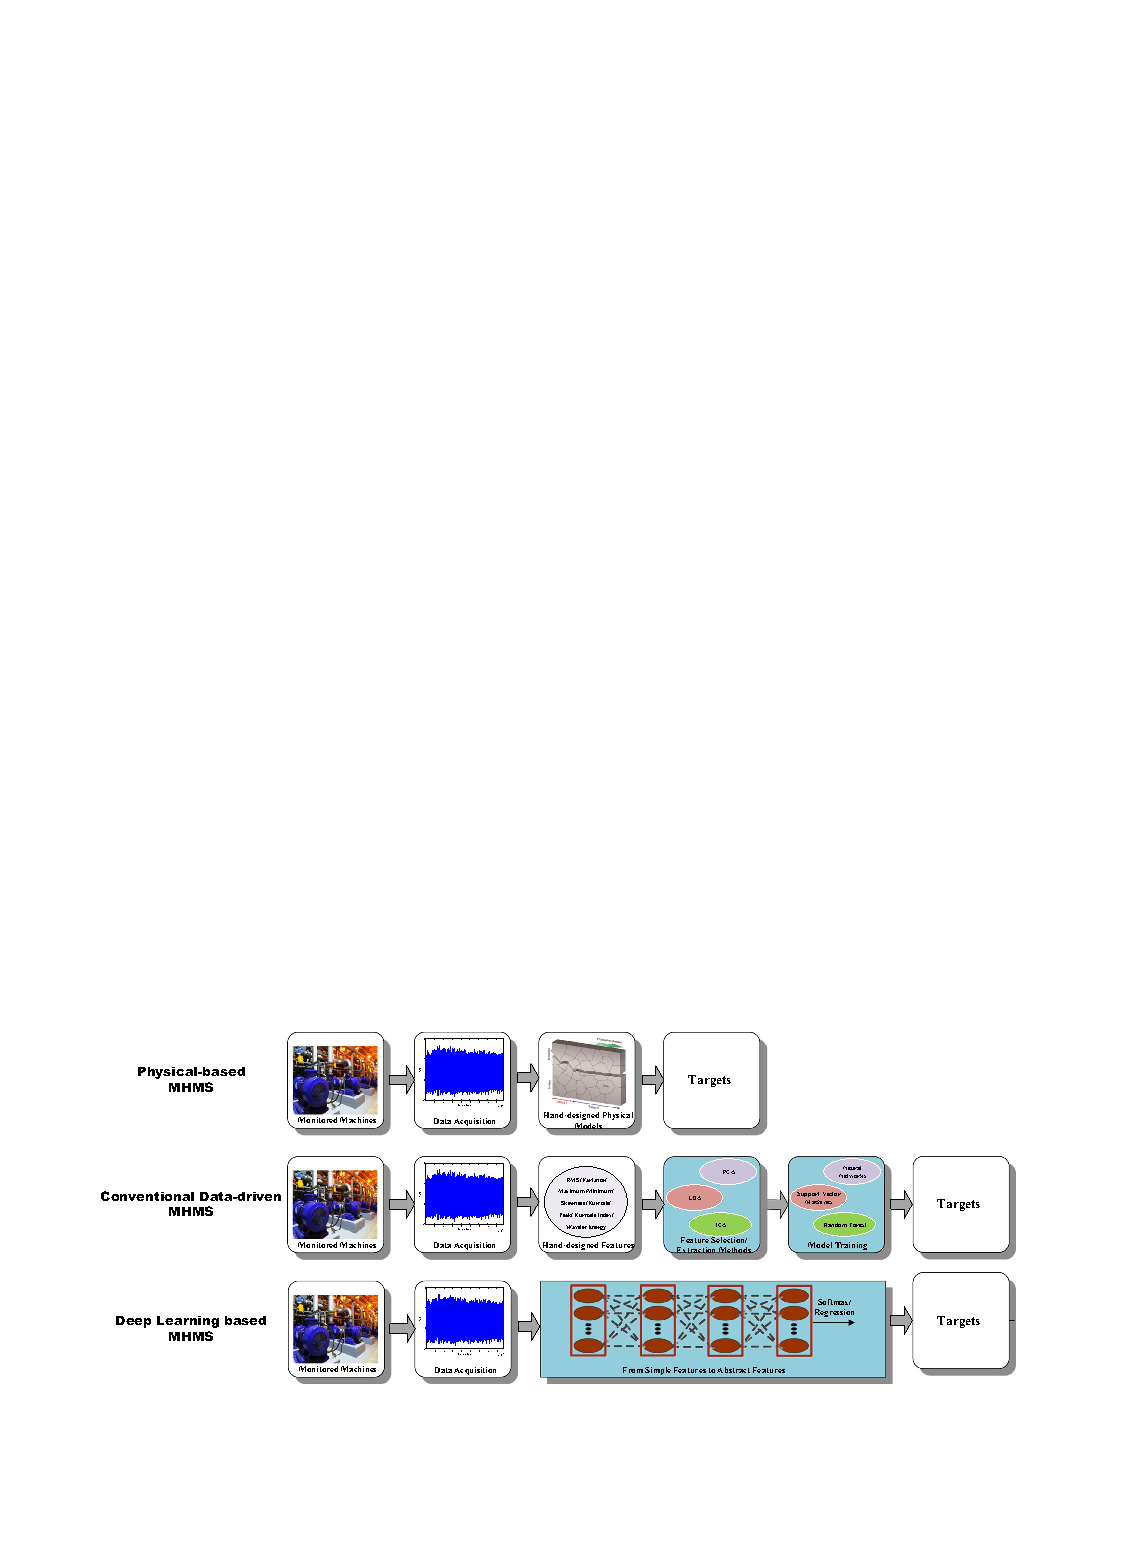
\includegraphics[width=1\textwidth]{hand_crafted_features_physical_models_deep_learning.pdf}
  \caption {Overview over traditional and deep learning-based PHM approaches \cite{ZHAO2019213}} \label{fig:hand_crafted_features_physical_models_deep_learning}
\end{figure}